\section{System Design}

The system design is task-driven. Before diving into the design of system, we introduce  the couple of tasks the system works for. 

\begin{itemize}
\item \textit{Identify the group of people with specific individual characteristics (T1)}: multiple attributes, semantic understanding, loose attribute boundary
\item \textit{Explore the mobility patterns of a group (T2)}: where those people go and how they access the ... in a city. the patterns of behaviour classified by different social characteristics, including travel demands. 
\item \textit{Compare mobility patterns among multiple groups (T3)}: what the similar and difference between groups in their traveling behaviour
\end{itemize}

Based on tasks, we derive the design considerations:

\begin{itemize}
\item \textit{C1: multivarible filter of individual characteristics}: Cross filter...
\textbf{C3: referrable transpotation}: TAZ
\item \textit{C2: intuitive understanding/combination understanding of individual characteristics}: since the concept of groups is vague to define directly quantitativily. The visual design needs to consider how to help end-users to pick desirable ones from the mass. 
\item \textit{C3: conventional travel analysis}: TAZ based
\item \textit{C4: multivariate analysis of mobility patterns in the constraint of spatial space}: the analysis of mobility patterns include multivariables, including the conventional spatial and temporal dimensions, as well as travel demands, frequency, etc.
\item \textit{C5: knowledgable, not too fractional findings}
\item \textit{C6: easy comparison}: 
\end{itemize}

Classification method, flow clustering method, Semantic representation. 

The key of our work is to align the analysis of urban dynamics with the available of demographic characteristics. 

Semantic understanding of social characteristics.

\subsection{Data-driven Profile Visualization}

Glyph-based visualization~\cite{borgo2013glyph} is the form of visual design to compose multivaribles into a collection of unified visual symbols, known as glyph. Glyph is intended for quick understanding and aligned comparison. Among glyph design, Chernoff Face~\cite{chernoff1973use} represents data variabules by the different features of a cartoon face. Following the idea of Chernoff Face~\cite{chernoff1973use}, we design a type of glyph, a graphical representation of people with specific demographic characteristics. The idea behind using faces is that humans easily recognize faces and notice small changes without difficulty. Those visual profiles are intended for intutive visual understanding and clustering, to abstract to concrete and semantic understanding, to help users clues to target the interested individual groups effectively.

Figure~\ref{fig:design_profile} shows the legend for the user profile. Those design dimensions are driven by data.The eight demographic dimensions are systematically designed into different visual symbols. Considering there are two types of variables, i.e., the numeric attributes and categorical attributes. By different composition, stimulus pattern which has the abstract deomgraphic measurement of individuals.

\begin{itemize}
\item \textbf{Gender} the gender is visually mapped to the hair style of the avatar. 
\item \textbf{Age} age is implied by the decoration on the hair. For the elder above 70, the hair is dyed to gray. For the youth beneath 18, hair decoration for girls and boys are adapted to the hair style.
\item \textbf{Education} The thickness of eye glasses is used to indicate the different levels in education.
\item \textbf{Job} The clothes is designed to imply the job of the individual. There are 9 types of clothes.
\item \textbf{Belongings} for house, car, residential license are considered as the belongings to the individual, so we design each of them as an add-on decoration to imply whether the individual has it or not.
\item \textbf{Income} a money symbol is used to show the different income levels.
\end{itemize} 

\begin{figure}[htb!]
 \centering % avoid the use of \begin{center}...\end{center} and use \centering instead (more compact)
 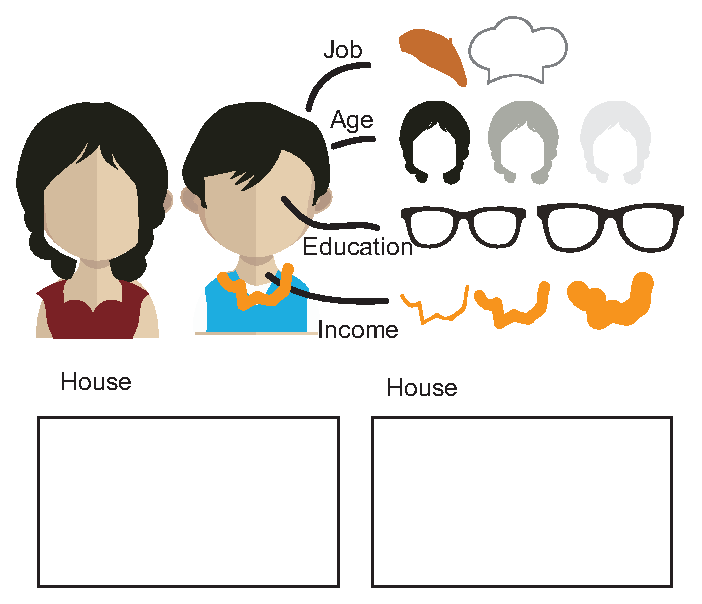
\includegraphics[width=\columnwidth]{pictures/design_profile}
 \caption{Design Profile}
 \label{fig:design_profile}
\end{figure}

With the visual mapping, the profiles varies from individual to individual. Figure~\ref{fig:div_profile} shows some examples. By concretizing the attributes which otherwise is too abstract to percept, users can scan and search for interesting target organically in figures.

\begin{figure}[htb!]
 \centering % avoid the use of \begin{center}...\end{center} and use \centering instead (more compact)
 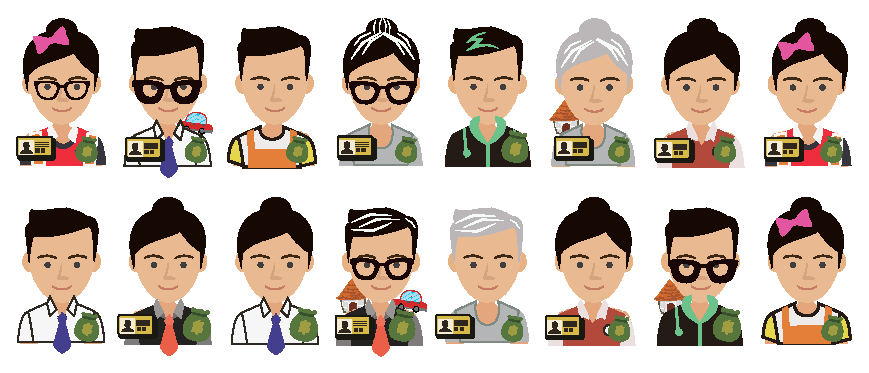
\includegraphics[width=\columnwidth]{pictures/design_div}
 \caption{Diverse Profile}
 \label{fig:div_profile}
\end{figure}

\subsection{t-SNE Projection}

Each individual is denoted as a vector with eight factors and projected as a dot into the 2D view via t-SNE project~\cite{maaten2008visualizing}, which well suits high-dimensional data for visualization in a low-dimensional space of two dimensions. As Figure~\ref{fig:tsne}(a)shows, all volunteers are embedded evenly in the 2D view, indicating the uniformly sampling over demographical space. 

Multiple views of abstract view, t-SNE proection and semantic data driven profile visualization are coordinated in a Cross-filter machinesm~\cite{Weaver2010}. It allows end-users to interactive drill-dowm into individuals with interested characteristics from multiple perspectives. Starting from the abstract criterion constraints, the scope of interest is narrowed down to individuals with(out) certian properties. And then further cross-filtering with semantically visual profiles, to check the combination of 8 characteristical variables. Figure~\ref{fig:tsne}(b) examplifies four groups of interest. 

\begin{figure}[htb!]
 \centering % avoid the use of \begin{center}...\end{center} and use \centering instead (more compact)
 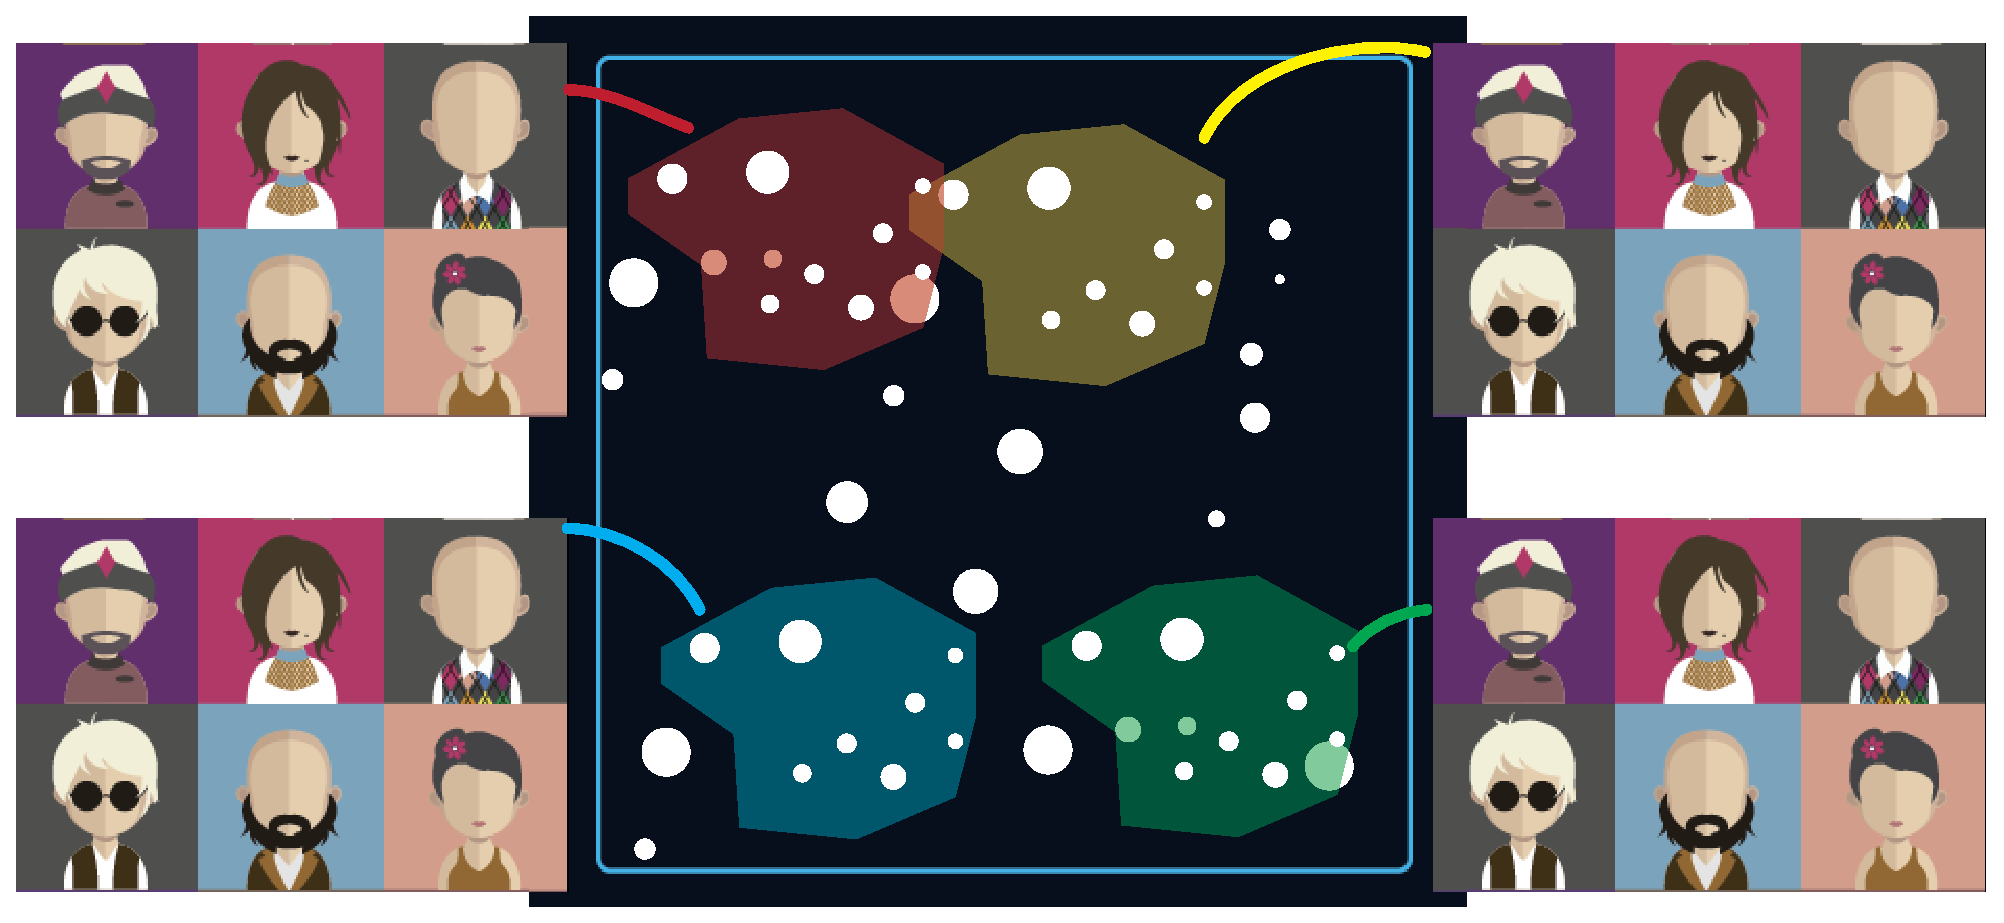
\includegraphics[width=\columnwidth]{pictures/mds}
 \caption{t-SNE project with four groups of the interest}
 \label{fig:tsne}
\end{figure}

\subsection{2.5D Spatial Visualization}

Embedding multiple variables in the spatial map is a challenging problem. Distortion technique 2D spatial, such as the partial route embedding~\cite{sun2016embedding}. However, when it comes to the global visualization, the trade-off between occlusion-free and the spatial perception. Follow the idea of 2.5D space design~\cite{Tominski2012_stacking}, the space visualization is embedded in 2.5D space, which also can smoothly transited back to the conventional 2D view.  

 Each TAZ is grown as a prism whose height encodes the occurrence of visiting. Brunch of TAZ with similar visiting pattern and purpose are grouped by an heuristic DB-Scan Algorithm in the context of TAZ. From a center TAZ, walk to neighbour TAZ to check whether aggregation or not. The aggregated TAZ brunch indicates the region visiting by the group of people in same purpose, which is often the popular traveling places. The TAZ brunch is visualized...

 To compare the mobility patterns across different groups of people, a Small Multiple dock is used to reserve the ever explored interesting result. To simply the comparion over spatial distribution, the snapshot is rendered in the 2D space, which can be magnified to check for the details in the 2.5D space.

 In this view, it supports end-users to direct manipulate the space, e.g., zooming, panning, etc. Also, detail information about the visiting can be checked by direct clicking on the TAZ. 